\chapter{Testes}\label{chp:testes}
Este capítulo visa descrever o procedimento de teste detalhando as ferramentas utilizadas para testar as partes do projeto individualmente, bem como a integração delas.

O grupo desenvolveu testes unitários de forma intensiva para garantir o correto funcionamento dos módulos do projeto. Para tanto, foram utilizadas algumas ferramentas de automação de testes. No primeiro sub-projeto, o grupo utilizou o Mocha\footnote{Disponível em \url{https://mochajs.org/}}, uma plataforma de execução de testes sobre Node.js (Figura \ref{fig:mocha_teste}). No segundo sub-projeto, duas ferramentas de teste foram utilizadas: o JUnit\footnote{Disponível em \url{http://junit.org/}} e o módulo embutido de testes da linguagem Clojure.

\begin{figure}[h]
	\centering
	\caption{Exemplo de teste unitário utilizando a ferramenta Mocha.}
  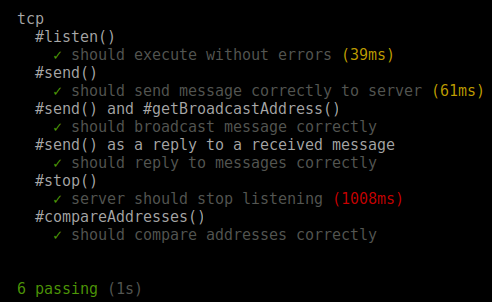
\includegraphics[width=0.7\textwidth]{imagens/mocha_teste.png}
  \label{fig:mocha_teste}  
\end{figure}

Os testes de integração foram efetuados desenvolvendo-se versões simplificadas, mas funcionalmente equivalentes, do componente a ser integrado. Como mencionado anteriormente, os módulos do projeto (dispositivos e controlador locais, servidor \textit{web} e aplicativo móvel) foram desenvolvidos de forma independente. Assim, para cada um desses componentes, foi desenvolvido um simulador que possibilitasse integrar com outro módulo a ser testado.

Para os dispositivos e controlador da rede local, foram desenvolvidos versões utilizando o protocolo TCP que podem ser executados no próprio computador; para o servidor, foram desenvolvidos bancos de dados de teste que simulassem o estado atual de uma residência, e para o aplicativo, foi implementada uma versão de depuração capaz de enviar e receber os comandos do protocolo Homecloud (Figura \ref{fig:aplicativo_teste}).

\begin{figure}[h]
	\centering
	\caption{Aplicativo utilizado nos testes de integração.}
  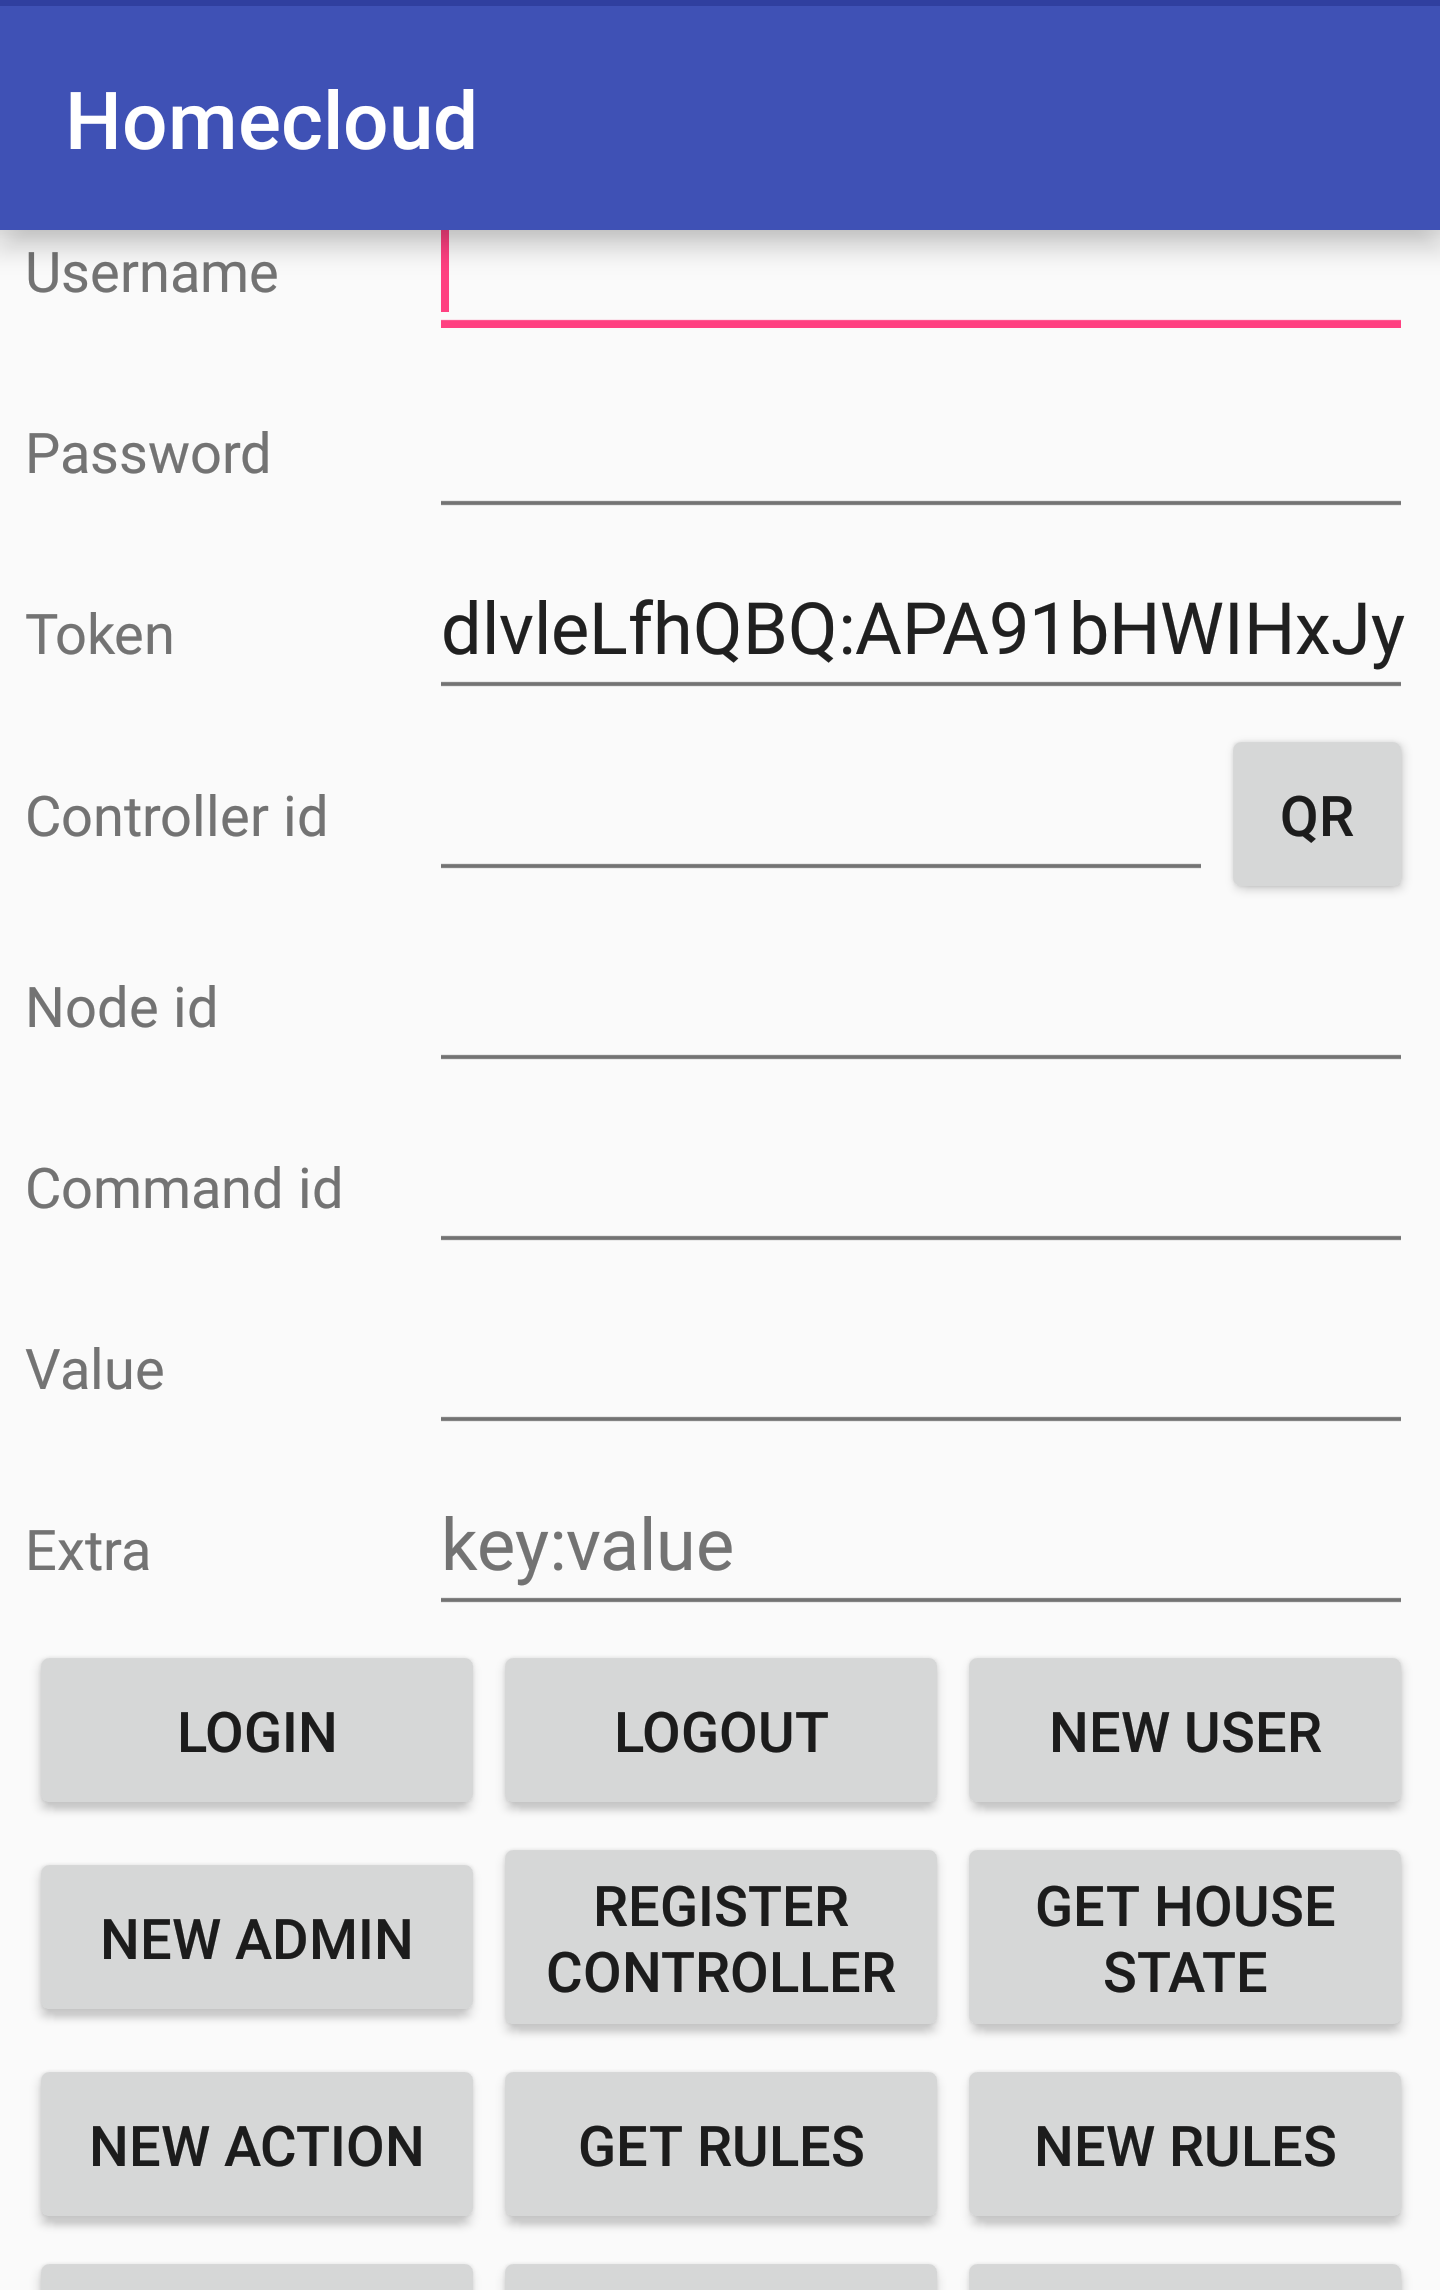
\includegraphics[width=0.5\textwidth]{imagens/aplicativo_teste.png}
  \label{fig:aplicativo_teste}  
\end{figure}
